\section{1174006 - Kadek Diva Krishna Murti}

\subsection{Teori}
\begin{enumerate}
	\item Jelaskan dengan ilustrasi gambar sendiri apa itu generator dengan perumpamaan anda sebagai mahasiswa sebagai generatornya.\\
    
    Generator merupakan jaringan yang menggunakan data yang ada (seperti gambar, video, audio, atau teks) untuk dijadikan data yang baru. Misalnya menggunakan gambar yang sudah ada untuk menghasilkan gambar yang baru. Tujuan utama generator adalah untuk menghasilkan data (seperti gambar, video, audio, atau teks) dari vektor angka yang dihasilkan secara acak. Perumpamaannya saya sebagai mahasiswa atau generator mengubah beberapa baris kodingan teman yang sudah ada. Sehingga menghasilkan kodingan yang baru.

    \begin{figure}[H]
	 	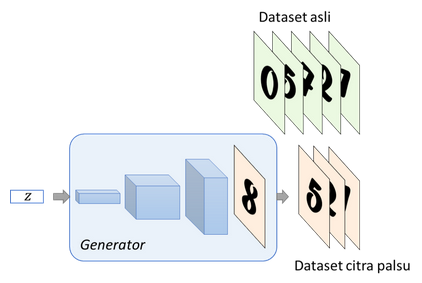
\includegraphics[width=6cm]{figures/1174006/chapter8/teori/1.png}
		\centering
    \end{figure}
    
	\item Jelaskan dengan ilustrasi gambar sendiri apa itu diskriminator dengan perumpamaan dosen anda sebagai diskriminatornya.\\
    
    Diskriminator merupakan jaringan yang mencoba membedakan antara data yang ada dengan data baru yang dihasilkan oleh generator.  Diskriminator mencoba memasukkan data inputan (data yang sudah ada) ke dalam kategori yang telah ditentukan. Perumpamaannya dosen atau dikriminator mencoba membedakan kodingan yang dibuat oleh saya dengan teman saya untuk menemukan kodingan yang mana yang sudah ada dan kodingan yang hasil perubahan.

    \begin{figure}[H]
        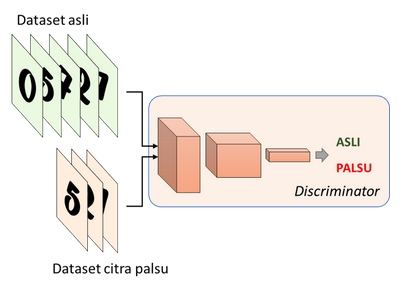
\includegraphics[width=6cm]{figures/1174006/chapter8/teori/2.png}
       \centering
   \end{figure}

	\item Jelaskan dengan ilustrasi gambar sendiri bagaimana arsitektur generator dibuat.\\
    Arsitektur generator:
    \begin{enumerate}
        \item Jaringan generator mencoba membuat data yang terlihat seperti data yang nyata dari data yang sudah ada.
        \item Ulangi langkah pertama hingga beberapa iterasi untuk mengecoh diskriminator dengan membuat data yang senyata mungkin.
        \item Hingga akhirnya, diskriminator melatih generator hingga ia tidak bisa lagi membedakan data nyata dan data yang palsu.
    \end{enumerate}

    \begin{figure}[H]
        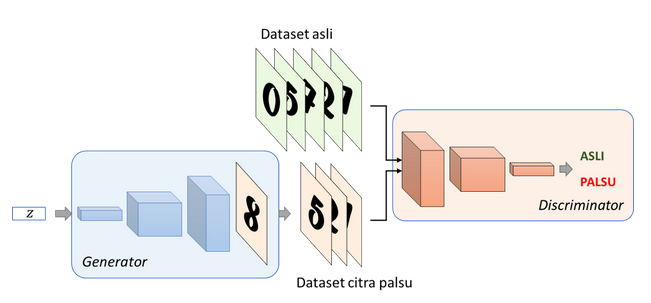
\includegraphics[width=6cm]{figures/1174006/chapter8/teori/3.PNG}
       \centering
   \end{figure}

	\item Jelaskan dengan ilustrasi gambar sendiri bagaimana arsitektur diskriminator
    dibuat.

    Arsitektur diskriminator:
    \begin{enumerate}
        \item Jaringan diskriminator mencoba mengidentifikasi apakah data tersebut asli atau palsu.
        \item Ulangi langkah pertama hingga beberapa iterasi untuk mengecoh generator dengan memperbaiki kriterianya untuk menentukan palsu tidaknya.
        \item Hingga akhirnya, diskriminator melatih generator hingga ia tidak bisa lagi membedakan data nyata dan data yang palsu.
    \end{enumerate}

    \begin{figure}[H]
        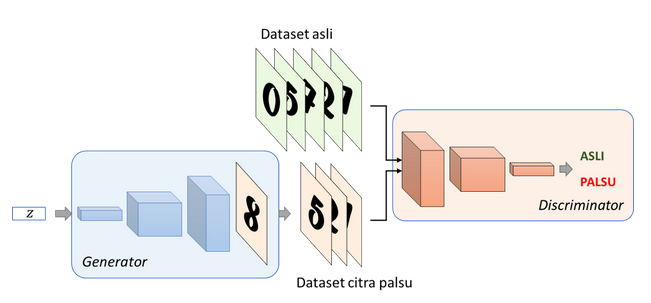
\includegraphics[width=6cm]{figures/1174006/chapter8/teori/3.PNG}
       \centering
   \end{figure}

    \item Jelaskan dengan ilustrasi gambar apa itu latent space.\\
    Latent space adalah data yang dibuat dari beberapa vektor secara acak.
    \begin{figure}[H]
        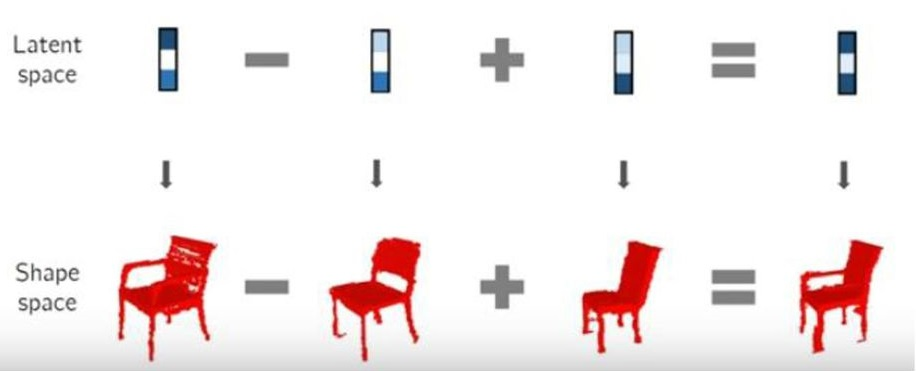
\includegraphics[width=6cm]{figures/1174006/chapter8/teori/4.jpg}
       \centering
   \end{figure}
    \item Jelaskan dengan ilustrasi gambar apa itu adversarial play.\\
    Adversarial play adalah proses pelatihan dimana jaringan discriminator dan jaringan generator berusaha saling memebodohi satu sama lain.
    
    \item Jelaskan dengan ilustrasi gambar apa itu Nash equilibrium.\\
    Nash Equilibrium adalah keadaan dimana jaringan discriminator tidak dapat membedakan lagi data asli dan data palsu.
    
    \item Sebutkan dan jelaskan contoh-contoh implementasi dari GAN.
    
    \begin{enumerate}
    	\item Image Generation, dimana GAN digunakan untuk mengenerate data baru dari perpaduan data asli yang ada.
    	\item Text to image synthesis, dimana GAN digunakan untuk mengenerate gambar berdasarkan deskripsi teks yang ada.
		\item Face aging, dimana GAN digunakan untuk mengenerate beberapa gambar wajah berbeda usia.
    	\item Image to image translation, dimana GAN digunakan untuk mengenerate gambar baru dari gambar yang sudah ada disertai dengan penambahan style.
		\item Video synthesis, dimana GAN digunakan untuk mengenerate sebuah video.
    	\item High resolution image generation, dimana GAN digunakan untuk meningkatkan resolusi atau mempertajam gambar.
    	\item Completing missing parts of images, dimana GAN digunakan untuk menambal bagian gambar yang hilang.
    \end{enumerate}
    
    
    \item Berikan contoh dengan penjelasan kode program beserta gambar arsitektur untuk membuat generator(neural network) dengan sebuah input layer, tiga hidden layer(dense layer), dan satu output layer(reshape layer).\\ \\
    Input Layer\\
    Pada input layer diambil sampel vertor 100 dimensi dan dilempar ke hidden layer pertama berupa tensor.\\
    \begin{lstlisting}
    input_shape=(batch_size, 100), output_shape=(batch_size, 100)
    \end{lstlisting}
    Hidden Layer\\
    Pada hidden layer akan ada proses konversi dari tensor yang dilempar dari layer sebelumnya. Pada hidden layer terdiri dari beberpa dense layer dengan beberapa unit juga.\\
    \begin{lstlisting}
    neurons=500, input_shape=(batch_size, 100), output_shape=(batch_size, 500)
    \end{lstlisting}
    \begin{lstlisting}
    neurons=500, input_shape=(batch_size, 500), output_shape=(batch_size, 500)
    \end{lstlisting}
    \begin{lstlisting}
    neurons=784, input_shape=(batch_size, 500), output_shape=(batch_size, 784)
    \end{lstlisting}
    Output Layer\\
    Pada output layer akan digenerate gambar yang memiliki bentuk 28 x 28 unit.\\
    \begin{lstlisting}
    input_shape=(batch_size, 784), output_shape=(batch_size, 28, 28)
    \end{lstlisting}
    \begin{figure}[H]
    	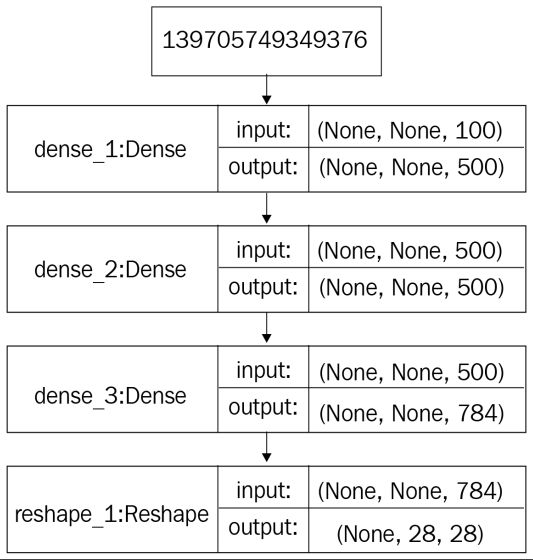
\includegraphics[width=6cm]{figures/1174006/chapter8/teori/arc.png}
    	\centering
    \end{figure}
    \item Berikan contoh dengan ilustrasi dari arsitektur dikriminator dengan sebuath input layer, 3 buah hidden layer, dan satu output layer.
    \begin{figure}[H]
    	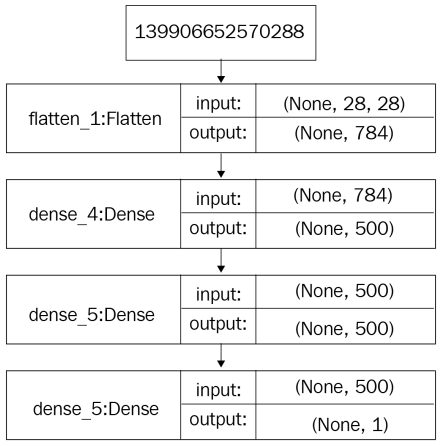
\includegraphics[width=6cm]{figures/1174006/chapter8/teori/arc2.png}
    	\centering
    \end{figure}
    \item Jelaskan bagaimana kaitan output dan input antara generator dan diskriminator tersebut. Jelaskan kenapa inputan dan outputan seperti itu.\\
    Inputan pada jaringan generator akan menerima input dari gambar asli, kemudian akan diolah oleh jaringan generator untuk dibuatkan gambar palsunya. Setelah dibuat gambar palsunya, kemudian akan diolah oleh jaringan diskriminator untuk dibedakan apakah gambar yang diolah sebelumnya oleh jaringan generator adalah asli atau palsu. Setelah diolah oleh jaringan discriminator akan mengembalikan value 0 atau 1
    
    \item Jelaskan apa perbedaan antara Kullback-Leibler divergence (KL divergence)/relative entropy, Jensen-Shannon(JS) divergence / information radius(iRaD) / total divergence to the average dalam mengukur kualitas dari model.\\
    Kullback-Leibler divergence tidak menerapkan symmetric nature untuk mengukur jarak antara dua probabilitas distribusi, sedangkan Jensen-Shannon divergence menerapkan symmetric nature.
    
    
    \item Jelaskan apa itu fungsi objektif yang berfungsi untuk mengukur kesamaan antara gambar yang dibuat dengan yang asli.\\
    Fungsi objektif berfungsi untuk mengukur kesamaan antara gambar yang dibuat dengan yang asli.
    
    \item Jelaskan apa itu scoring algoritma selain mean square error atau cross entropy seperti The Inception Score dan The Frechet Inception distance.\\
    Scoring algoritma adalah algoritma yang digunakan untuk menghitung akurasi GAN.
    
    \item Jelaskan kelebihan dan kekurangan GAN.\\
    Kelebihan
    \begin{enumerate}
    	\item Data hasil generate GAN terlihat mirip dengan data asli.
		\item Gampang dalam mengenali suatu objek dan bisa menghitung jarak antar objek
    \end{enumerate}
    Kekurangan
    \begin{enumerate}
    	\item Susah untuk dilatih
    \end{enumerate}

\end{enumerate}

\subsection{Praktek}
\begin{enumerate}
	\item Jelaskan apa itu 3D convolutions\\
	3D convolution adalah operasi menerapkan filter 3D ke data input sepanjang tiga arah, yaitu x, y, z. Operasi akan membuat daftar 3D fitur secara bertumpuk, outputnya nanti berupa kotak.
	
	\item Jelaskan dengan kode program arsitektur dari generator networknya, beserta penjelasan input dan output dari generator network.
	\\ \\
	Input Layer\\
	Pada input layer diambil sampel vertor 100 dimensi dan dilempar ke hidden layer pertama berupa tensor.\\
	\begin{lstlisting}
	input_shape=(batch_size, 100), output_shape=(batch_size, 100)
	\end{lstlisting}
	Hidden Layer\\
	Pada hidden layer akan ada proses konversi dari tensor yang dilempar dari layer sebelumnya. Pada hidden layer terdiri dari beberpa dense layer dengan beberapa unit juga.\\
	\begin{lstlisting}
	neurons=500, input_shape=(batch_size, 100), output_shape=(batch_size, 500)
	\end{lstlisting}
	\begin{lstlisting}
	neurons=500, input_shape=(batch_size, 500), output_shape=(batch_size, 500)
	\end{lstlisting}
	\begin{lstlisting}
	neurons=784, input_shape=(batch_size, 500), output_shape=(batch_size, 784)
	\end{lstlisting}
	Output Layer\\
	Pada output layer akan digenerate gambar yang memiliki bentuk 28 x 28 unit.\\
	\begin{lstlisting}
	input_shape=(batch_size, 784), output_shape=(batch_size, 28, 28)
	\end{lstlisting}
	\begin{figure}[H]
		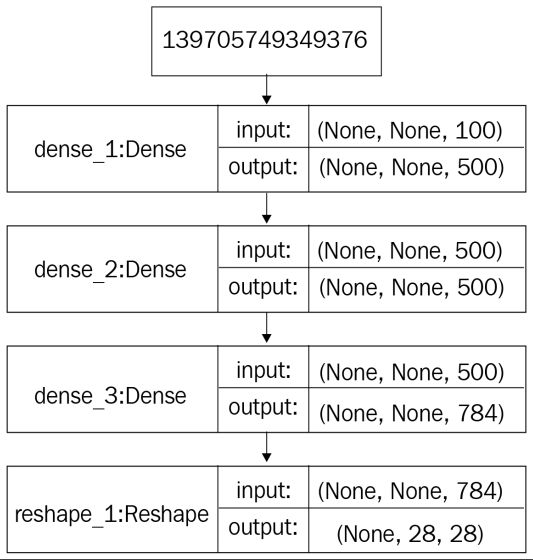
\includegraphics[width=6cm]{figures/1174006/chapter8/teori/arc.png}
		\centering
	\end{figure}

	\item Jelaskan dengan kode program arsitektur dari diskriminator network, beserta penjelasan input dan outputnya.
	\\ \\
	Input Layer\\
	Pada input layer diambil sampel vertor 100 dimensi dan dilempar ke hidden layer pertama berupa tensor.\\
	\begin{lstlisting}
	input_shape=(batch_size, 100), output_shape=(batch_size, 100)
	\end{lstlisting}
	Hidden Layer\\
	Pada hidden layer akan ada proses konversi dari tensor yang dilempar dari layer sebelumnya. Pada hidden layer terdiri dari beberpa dense layer dengan beberapa unit juga.\\
	Pertama dicriminator akan menerima inputan bentuk 28 x 28. Lalu diteruskan ke hidden layer tanpa dimodifikasi. Pada hidden layer akan dimodifikasi. Lalu pada layer terakhir atau output layer ditentukan apakah data tadi adalah asli atau palsu
	\begin{figure}[H]
		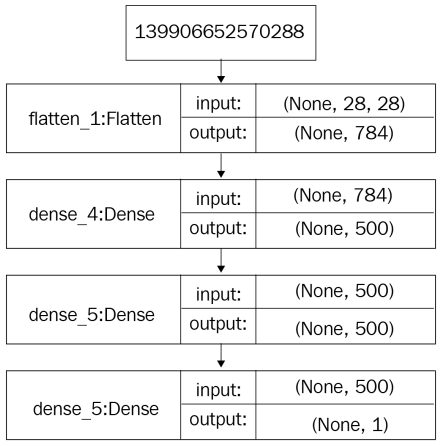
\includegraphics[width=6cm]{figures/1174006/chapter8/teori/arc2.png}
		\centering
	\end{figure}
	\item Jelaskan proses training 3D-GANs.
	\begin{enumerate}
		\item Siapkan sample 200 dimensi berbentuk vektor.
		\item Generate sebuah gambar palsu dengan model generator.
		\item Latih jaringan generator dengan gambar asli dan gambar palsu.
		\item Gunakan adversial model untuk melatih generator model.
		\item Ulangi langkah diatas sampai epoch tertentu.
		
	\end{enumerate}
	\item Jelaskan bagaimana melakukan settingan awal chapter 02 untuk memenuhi semua kebutuhan sebelum melanjutkan ke tahapan persiapan data.
	\begin{enumerate}
		\item Download terlebih dahulu data yang akan diolah
		\item Siapkan IDE yang akan dipakai untuk mengolah data.
		\item Panggil data yang telah didownload tadi.
	\end{enumerate}
	\item Jelaskan tentang dataset yang digunakan, dari mulai tempat unduh, cara membuka dan melihat data. Sampai deskripsi dari isi dataset dengan detail penjelasan setiap folder/file yang membuat orang awam paham.
	\begin{enumerate}
		\item Pertama download dataset dengan mengetik wget http://3dshapenets.cs.princeton.edu/3DShapeNetsCode.zip
		\item Lalu extract dataset tadi dengan mengetik unzip 3DShapeNetsCode.zip
		\item Panggil data yang telah didownload tadi.
	\end{enumerate}
	\item Jelaskan apa itu voxel dengan ilustrasi dan bahasa paling awam.\\
	Voxel adalah point pada bentuk 3 dimesional, biasanya berup posisi dari 3 koordinat yaitu x, y, dan z.
	
	\item Visualisasikan dataset tersebut dalam tampilan visual plot, jelaskan cara melakukan visualisasinya.
	\begin{enumerate}
		\item Pertama load data gambar 3D.
		\item Lalu visualisasikan data gambar 3D tadi.
	\end{enumerate}
	\begin{figure}[H]
		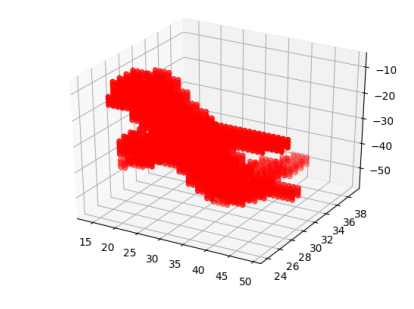
\includegraphics[width=6cm]{figures/1174006/chapter8/praktek/ex.png}
		\centering
	\end{figure}
	
	\item Buka file run.py jelaskan perbaris kode pada fungsi untuk membuat generator yaitu build generator.\\
	Pada kode fungsi build\_generator() dibuat untuk nantinya dipakai sebagai model generator. Di fungsi tersebut berisikan layer-layer yang terla di definisikan sesuai keperluan generator.
	
	\item Jelaskan juga fungsi untuk membangun diskriminator pada fungsi build discriminator.\\
	Pada kode fungsi build\_discriminator() dibuat untuk nantinya dipakai sebagai model discriminator. Di fungsi tersebut berisikan layer-layer yang terla di definisikan sesuai keperluan discriminator.
	
	\item Jelaskan apa maksud dari kode program \_\_name\_\_ == '\_\_main\_\_'
    \begin{lstlisting}[caption=Kode program utama,label={lst:8.1}]
    if __name__ == '__main__':
    \end{lstlisting}
    Kode program tersebut untuk mengecek apakah module yang dipakai adalah main.
    
    \item Jelaskan secara detil perbaris dan per parameter apa arti dari kode program :
    \begin{lstlisting}[caption=Setting Parameter,label={lst:8.2}]
        object_name = "chair"
        data_dir = "data/3DShapeNets/volumetric_data/" \
                "{}/30/train/*.mat".format(object_name)
        gen_learning_rate = 0.0025
        dis_learning_rate = 10e-5
        beta = 0.5
        batch_size = 1
        z_size = 200
        epochs = 10
    \end{lstlisting}
    Kode program diatas tentang mendefinisikan variable yang akan dipakai.
    
    \item Jelaskan secara detil dari kode program pembuatan dan kompilasi arsitektur berikut :
    \begin{lstlisting}[caption=Setting Parameter,label={lst:8.2}]
        gen_optimizer = Adam(lr=gen_learning_rate, beta_1=beta)
        dis_optimizer = Adam(lr=dis_learning_rate, beta_1=beta)

        discriminator = build_discriminator()
        discriminator.compile(loss='binary_crossentropy', optimizer=dis_optimizer)

        generator = build_generator()
        generator.compile(loss='binary_crossentropy', optimizer=gen_optimizer)
    \end{lstlisting}
    Kode program diatas tentang pembuatan dan kompilasi model generator dan discriminator yang nantinya dipakai.
    
    \item Jelaskan secara detil kode program untuk membuat dan melakukan kompilasi model adversarial berikut:
    \begin{lstlisting}[caption=Membuat dan Kompilasi Model Adversarial,label={lst:8.3}]
        discriminator.trainable = False

        input_layer = Input(shape=(1, 1, 1, z_size))
        generated_volumes = generator(input_layer)
        validity = discriminator(generated_volumes)
        adversarial_model = Model(inputs=[input_layer], outputs=[validity])
        adversarial_model.compile(loss='binary_crossentropy', optimizer=gen_optimizer)
    \end{lstlisting}
    Kode program diatas tentang pembuatan dan kompilasi model adversial yang nantinya dipakai.
    
    \item Jelaskan Ekstrak dan load data kursi dengan menggunakan fungsi getVoxelsFormat dan get3DImages yang digunakan pada kode program berikut :
    \begin{lstlisting}[caption=Ekstraksi dan load dataset,label={lst:8.4}]
        print("Loading data...")
        volumes = get3DImages(data_dir=data_dir)
        volumes = volumes[..., np.newaxis].astype(np.float)
        print("Data loaded...")
    \end{lstlisting}
    Kode program diatas tentang meload data gambar 3D.
    
    \item Jelaskan maksud dari kode program instansiasi TensorBoard yang menambahkan generator dan diskriminator pada program berikut:
    \begin{lstlisting}[caption=Instansiasi tensorboard,label={lst:8.5}]
        tensorboard = TensorBoard(log_dir="logs/{}".format(time.time()))
        tensorboard.set_model(generator)
        tensorboard.set_model(discriminator)
    \end{lstlisting}
    Kode program diatas tentang mengevaluasi model yang dibuat dengan menggunakan TensorBoard.
    
    \item Jelaskan apa fungsi dari np reshape ones zeros pada kode program berikut dengan parameternya:
    \begin{lstlisting}[caption=Pelabelan dataset,label={lst:8.6}]
        labels_real = np.reshape(np.ones((batch_size,)), (-1, 1, 1, 1, 1))
        labels_fake = np.reshape(np.zeros((batch_size,)), (-1, 1, 1, 1, 1))
    \end{lstlisting}
    Kode program diatas tentang pelabelan data asli dan palsu.
    
    \item Jelaskan kenapa harus ada perulangan dalam meraih epoch. Dan jelaskan apa itu epoch terkait kode program berikut:
    \begin{lstlisting}[caption=Setting Epoch,label={lst:8.7}]
            for epoch in range(epochs):
                print("Epoch:", epoch)

                gen_losses = []
                dis_losses = []
    \end{lstlisting}
    Epoch dilakukan untuk mendapat hasil yang akurat. Kode program diatas tentang menampung tinggkat loss dari generator dan discriminator.
    
    \item Jelaskan apa itu batches dan kaitannya dengan kode program berikut, dan kenapa berada di dalam epoch:
    \begin{lstlisting}[caption=Setting Batch,label={lst:8.8}]
                number_of_batches = int(volumes.shape[0] / batch_size)
                print("Number of batches:", number_of_batches)
                for index in range(number_of_batches):
                    print("Batch:", index + 1)
    \end{lstlisting}
    Batch dipakai terkait pembagian proses pada tiap epoch yang dilakukan.
    
    \item Berikut adalah kode program pengambilan gambar dan noise. Jelaskan apa fungsi np.random.normal serta astype, serta jelaskan apa arti parameter titik dua dan jelaskan isi dari z\_sample dan volumes\_batch:
    \begin{lstlisting}[caption=Set real images dan vektor noise,label={lst:8.9}]
                    z_sample = np.random.normal(0, 0.33, size=[batch_size, 1, 1, 1, z_size]).astype(np.float32)
                    volumes_batch = volumes[index * batch_size:(index + 1) * batch_size, :, :, :]
    \end{lstlisting}

    \item Berikut adalah kode program generator gambar palsu. Jelaskan apa fungsi generator.predict\_on\_batch, serta jelaskan apa arti parameter z\_sample:
    \begin{lstlisting}[caption=Generator Gambar Palsu,label={lst:8.10}]
                    # Next, generate volumes using the generate network
                    gen_volumes = generator.predict_on_batch(z_sample)
    \end{lstlisting}

    \item Berikut adalah kode program training diskriminator dengan gambar palsu dari generator dan gambar asil. Jelaskan apa maksudnya harus dilakukan training diskriminator secara demikian dan jelaskan apa isi loss\_fake dan loss\_real serta d\_loss dan fungsi train\_on\_batch.
    \begin{lstlisting}[caption=Training Diskriminator,label={lst:8.11}]
                    discriminator.trainable = True
                    if index % 2 == 0:
                        loss_real = discriminator.train_on_batch(volumes_batch, labels_real)
                        loss_fake = discriminator.train_on_batch(gen_volumes, labels_fake)

                        d_loss = 0.5 * np.add(loss_real, loss_fake)
                        print("d_loss:{}".format(d_loss))

                    else:
                        d_loss = 0.0
    \end{lstlisting}

    \item Berikut adalah kode program training model adversarial yang terdapat generator dan diskriminator. Jelaskan apa bagaimana proses terbentuknya parameter z dan g\_loss:
    \begin{lstlisting}[caption=Training adversarial model,label={lst:8.12}]
                    z = np.random.normal(0, 0.33, size=[batch_size, 1, 1, 1, z_size]).astype(np.float32)
                    g_loss = adversarial_model.train_on_batch(z, labels_real)
                    print("g_loss:{}".format(g_loss))

                    gen_losses.append(g_loss)
                    dis_losses.append(d_loss)
    \end{lstlisting}

    \item Berikut adalah kode program generate dan menyimpan gambar 3D setelah beberapa saat setiap epoch. Jelaskan mengapa ada perulangan dengan parameter tersebut, serta jelaskan arti setiap variabel beserta perlihatkan isinya dan artikan isinya :
    \begin{lstlisting}[caption=Buat dan simpan gambar 3D,label={lst:8.13}]
                    # Every 10th mini-batch, generate volumes and save them
                    if index % 10 == 0:
                        z_sample2 = np.random.normal(0, 0.33, size=[batch_size, 1, 1, 1, z_size]).astype(np.float32)
                        generated_volumes = generator.predict(z_sample2, verbose=3)
                        for i, generated_volume in enumerate(generated_volumes[:5]):
                            voxels = np.squeeze(generated_volume)
                            voxels[voxels < 0.5] = 0.
                            voxels[voxels >= 0.5] = 1.
                            saveFromVoxels(voxels, "results/img_{}_{}_{}".format(epoch, index, i))
    \end{lstlisting}

    \item Berikut adalah kode program menyimpan average losses setiap epoch. Jelaskan apa itu tensorboard dan setiap parameter yang digunakan pada kode program ini :
    \begin{lstlisting}[caption=Simpan Average losses setiap epoch,label={lst:8.14}]
                # Write losses to Tensorboard
                write_log(tensorboard, 'g_loss', np.mean(gen_losses), epoch)
                write_log(tensorboard, 'd_loss', np.mean(dis_losses), epoch)
    \end{lstlisting}

    \item Berikut adalah kode program menyimpan model. Jelaskan apa itu format h5 dan penjelasan dari kode program berikut :
    \begin{lstlisting}[caption=Simpan model,label={lst:8.15}]
            generator.save_weights(os.path.join("models", "generator_weights.h5"))
            discriminator.save_weights(os.path.join("models", "discriminator_weights.h5"))
    \end{lstlisting}

    \item Berikut adalah kode program testing model. Jelaskan dengan ilustrasi gambar dari mulai meload hingga membuat gambar 3D dengan menggunakan z\_sample, bisakah parameter z\_sample tersebut diubah2? :
    \begin{lstlisting}[caption=Testing model,label={lst:8.16}]
            # Create models
            generator = build_generator()
            discriminator = build_discriminator()

            # Load model weights
            generator.load_weights(os.path.join("models", "generator_weights.h5"), True)
            discriminator.load_weights(os.path.join("models", "discriminator_weights.h5"), True)

            # Generate 3D models
            z_sample = np.random.normal(0, 1, size=[batch_size, 1, 1, 1, z_size]).astype(np.float32)
            generated_volumes = generator.predict(z_sample, verbose=3)

            for i, generated_volume in enumerate(generated_volumes[:2]):
                voxels = np.squeeze(generated_volume)
                voxels[voxels < 0.5] = 0.
                voxels[voxels >= 0.5] = 1.
                saveFromVoxels(voxels, "results/gen_{}".format(i))
    \end{lstlisting}
    
\end{enumerate}

\subsection{Penanganan Error}
\begin{enumerate}
	\item Screenshoot Error
	\item Tuliskan kode eror dan jenis errornya
	\item Solusi pemecahan masalah error tersebut
    
\end{enumerate}